\documentclass[a4paper, 12pt, UTF8]{article}

\usepackage{xeCJK}
\setCJKmainfont[BoldFont={SimHei},ItalicFont={KaiTi}]{SimSun}

\usepackage{amsfonts}
\usepackage{amsmath}
\usepackage{graphicx}
\usepackage{indentfirst}
\usepackage{listings}
\lstset{
    columns=flexible,
    breakatwhitespace=false,
    breaklines=true,
    frame=single,
    numbers=left,
    numbersep=5pt,
    showspaces=false,
    showstringspaces=false,
    showtabs=false,
    stepnumber=1,
    rulecolor=\color{black},
    tabsize=2,
    texcl=true,
    escapeinside={\%*}{*)},
    extendedchars=false,
    mathescape=true,
}

\usepackage[colorlinks, citecolor=red]{hyperref}

\setlength{\evensidemargin}{-0.05in}
\setlength{\oddsidemargin}{-0.05in}
\setlength{\headheight}{-0.2in}
\setlength{\headsep}{0in}
\setlength{\textheight}{9.75in}
\setlength{\textwidth}{6.5in}
\setlength{\parindent}{2em}

\renewcommand{\baselinestretch}{1.5}

\begin{document}

\title{计算机视觉第1次作业}
\author{黎健成}
\date{2015210936}
\maketitle

%-----
\section{实验目的}

\begin{enumerate}

\item 熟悉RGB、HSV、CIELab颜色空间、直方图。

\item 利用HSV(或RGB,CIELab)颜色直方图,进行基于颜色的图像检索。

\end{enumerate}


\section{实验要求}

\begin{enumerate}

\item 取四张图片,画出三种模型下的颜色直方图。

RGB:各通道256级。

HSV:H通道灰度级180,S通道灰度级256。

CIElab:忽略亮度L通道,并且将a及b通道量化为50个区间。

\item 采用RGB, HSV量化,累加直方图,CCV,Centering refinement,Color Coherence Distance Refinement进行图像检索。

\end{enumerate}

{\large 注意}

\begin{itemize}

\item 相似性度量:采用Correlation、直方图相交Intersection、开方统计Chi-Square statistic、巴式距离Bhattacharyya四种方法进行相似性度量。

\item HSV的区域2分为8个灰度区。

\item 采用OpenCV和Matlab或其它方法均可。

\item 注意颜色空间的转换方式以及图像文件的读取。

\end{itemize}


\section{实验环境}

操作系统:Windows 10

开发环境:Python 2.7.11 + OpenCV 3.1.0

Python Library:

\begin{itemize}

\setlength{\itemsep}{0pt}

\item numpy 1.10.4

\item matplotlib 1.5.1

\item Pillow 3.1.1

\end{itemize}

\section{实验过程}

\subsection{查看不同颜色空间的编码方式}

具体实现见\lstinline[language=bash]{hw1.py的demo1()}。

\begin{enumerate}

\item 给定的彩色JPG图片如图[\ref{figure_1}]。其中,彩色条块的RGB值分别为(255, 0, 0), (0, 255, 0), (0, 0, 255), (255, 0, 0), (0, 255, 0), (0, 0, 255),灰色方块值为(50, 50, 50), (150, 150, 150), (200, 200, 200)。

\begin{figure}[h!]
    \centering
    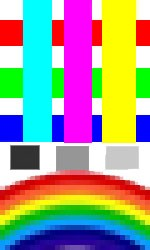
\includegraphics[width=0.2\textwidth]{in/1.jpg}
    \caption{1.jpg}
    \label{figure_1}
\end{figure}

\item 输出RGB颜色空间的通道数值。

如图[\ref{figure_demo1_B}]为B通道的数值。其在红、绿、黄区域的值为0,而在白、蓝、洋红等区域的值为255,在三个灰色方块区域则分别约为50,150,200。

\begin{figure}[h!]
    \centering
    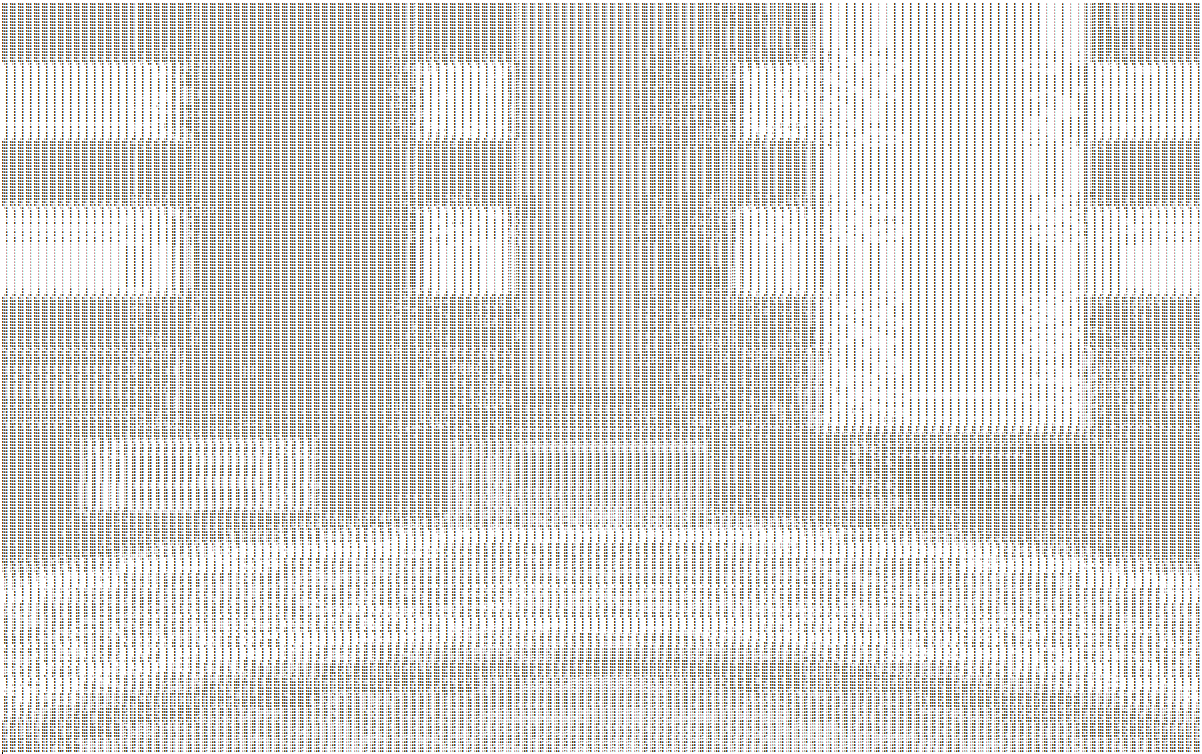
\includegraphics[width=0.8\textwidth]{out/demo1_B.png}
    \caption{B通道的数值}
    \label{figure_demo1_B}
\end{figure}

\item 输出HSV颜色空间的通道数值。

如图[\ref{figure_demo1_H}]为H通道的数值。虽然设计上HSV颜色空间的H通道取值范围是[0, 359],但在OpenCV中,通过自带的cvtColor函数转换的H数值范围为[0, 179]。其原因是测试图像的格式为8UC3,每通道仅8位,最大表示值255,故在存储H通道时其数值均被除以2后保存。如红色区域的值依然为0,绿色区域值则变为90,洋红区域为150等。

\begin{figure}[h!]
    \centering
    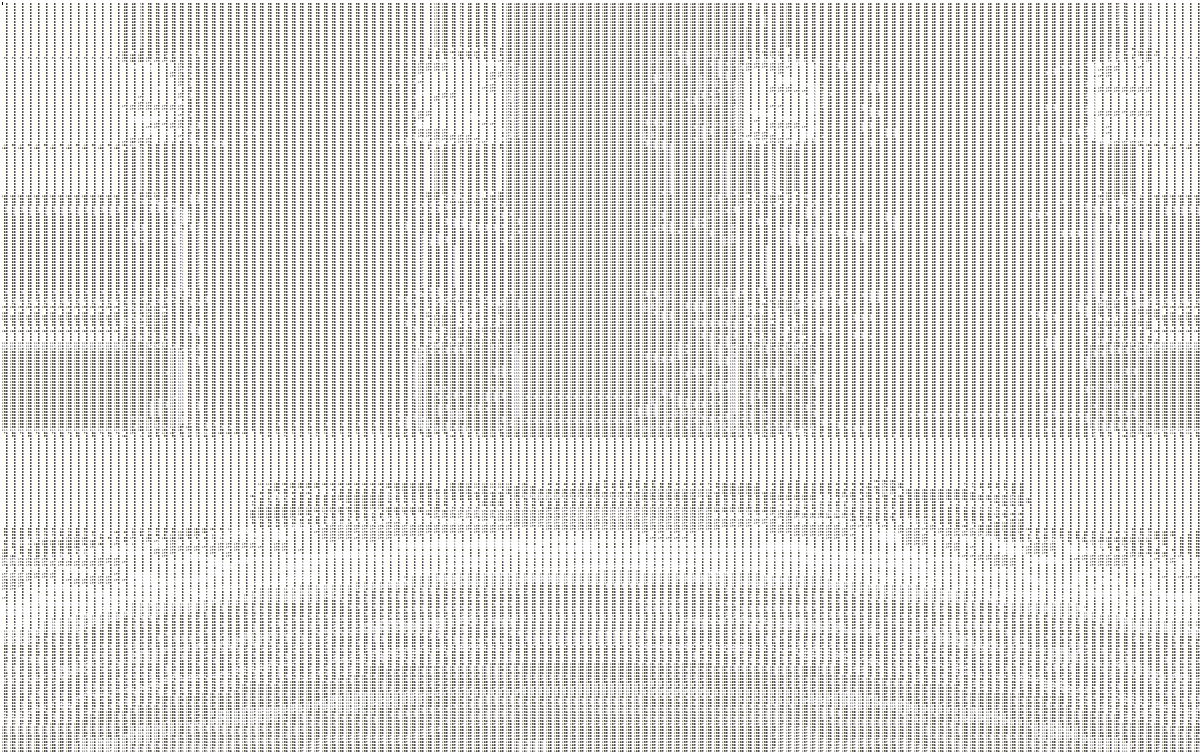
\includegraphics[width=0.8\textwidth]{out/demo1_H.png}
    \caption{H通道的数值}
    \label{figure_demo1_H}
\end{figure}

\item 输出CIELab颜色空间的通道数值。

如图[\ref{figure_demo1_a-}]为a*通道的数值。

\begin{figure}[h!]
    \centering
    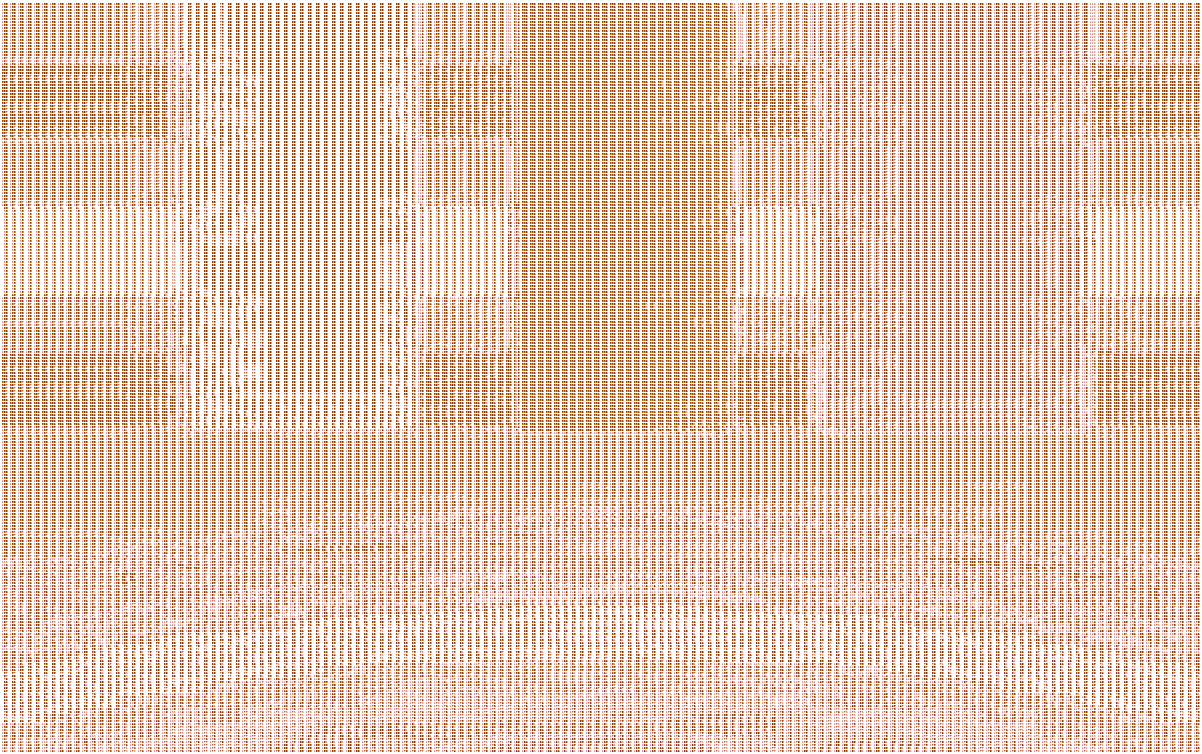
\includegraphics[width=0.8\textwidth]{out/demo1_a-.png}
    \caption{a*通道的数值}
    \label{figure_demo1_a-}
\end{figure}

\end{enumerate}

\clearpage

\subsection{画出不同颜色空间的颜色直方图}

具体实现见\lstinline[language=bash]{hw1.py的demo2()}。

\begin{enumerate}

\item 给定的4张图片如图[\ref{figure_4}]。

\begin{figure}[h!]
    \centering
    \begin{tabular}{cc}
        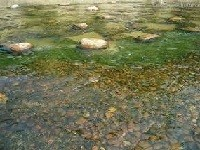
\includegraphics[width=0.3\textwidth]{in/r1.jpg} &
        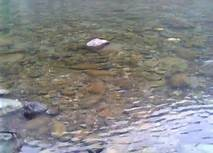
\includegraphics[width=0.3\textwidth]{in/r2.jpg} \\
        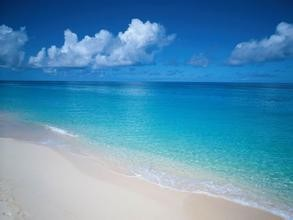
\includegraphics[width=0.3\textwidth]{in/s1.jpg} &
        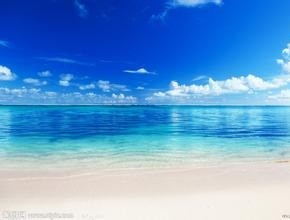
\includegraphics[width=0.3\textwidth]{in/s2.jpg}
    \end{tabular}
    \caption{给定的4张图片}
    \label{figure_4}
\end{figure}

\item 画出RGB颜色空间的颜色直方图。

如图[\ref{figure_demo2_r1_RGB}]为图片r1.jpg在RGB颜色空间各通道256级的颜色直方图。

\begin{figure}[h!]
    \centering
    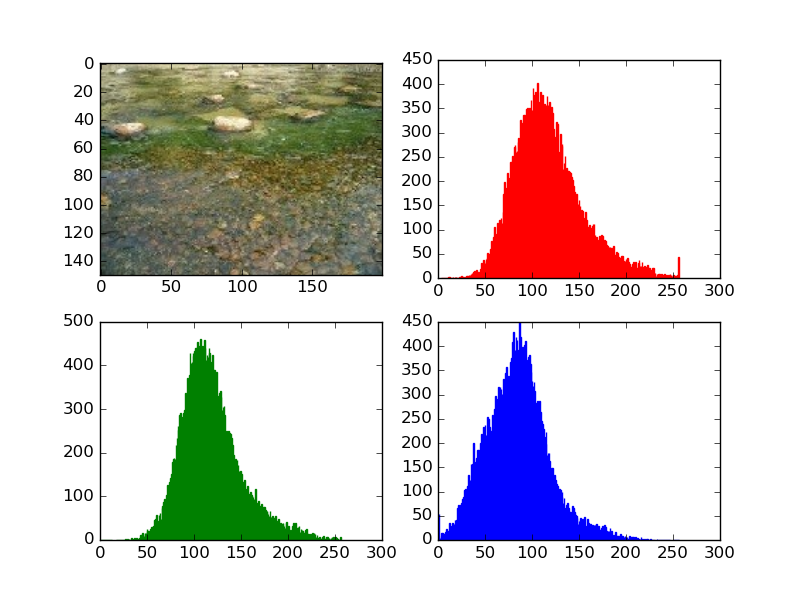
\includegraphics[width=0.7\textwidth]{out/demo2_r1_RGB.png}
    \caption{r1.jpg在RGB颜色空间各通道的颜色直方图}
    \label{figure_demo2_r1_RGB}
\end{figure}

\item 画出HSV颜色空间的颜色直方图。

如图[\ref{figure_demo2_r1_HSV}]为图片r1.jpg在HSV颜色空间各通道的颜色直方图,其中H通道180级,S通道256级。

\begin{figure}[h!]
    \centering
    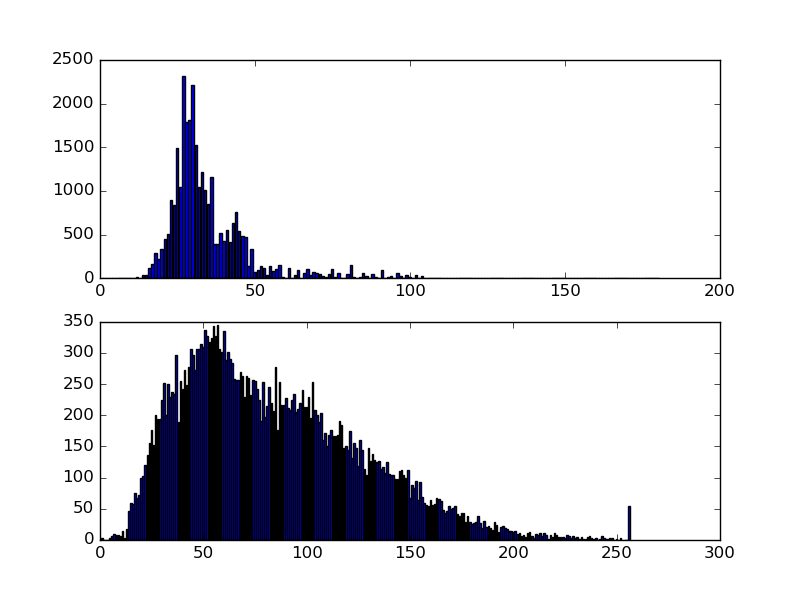
\includegraphics[width=0.7\textwidth]{out/demo2_r1_HSV.png}
    \caption{r1.jpg在HSV颜色空间各通道的颜色直方图}
    \label{figure_demo2_r1_HSV}
\end{figure}

\item 画出HSV颜色空间的颜色直方图。

如图[\ref{figure_demo2_r1_Lab}]为图片r1.jpg在CIELab颜色空间a*和b*通道的颜色直方图,其中忽略亮度L通道,并且将a*及b*通道量化为50个区间。

\begin{figure}[h!]
    \centering
    \includegraphics[width=0.7\textwidth]{out/demo2_r1_Lab.png}
    \caption{r1.jpg在CIELab颜色空间a*和b*通道的颜色直方图}
    \label{figure_demo2_r1_Lab}
\end{figure}

\end{enumerate}


\subsection{相似性度量}

采用Correlation、Intersection、Chi-Square statistic、Bhattacharyya四种方法进行相似性度量。前两者数值越大越相似,后两者数值越小越相似。

比较图片对分别使用r1.jpg自身比较、r1.jpg与r2.jpg、s1.jpg与s2.jpg、r1.jpg与s1.jpg、r2.jpg与s2.jpg。

具体实现见\lstinline[language=bash]{hw1.py的demo3()}。

\begin{enumerate}

\item RGB直方图对比

结果如表1-5所示。

\begin{table}[h!]
    \centering
    \caption{r1.jpg, r1.jpg}
    \begin{tabular}{ccccc}
        methods & Correlation & Intersection & Chi-Square & Bhattacharyya \\ \hline
        B通道 & 1.0 & 10.63 & 0.0 & 0.0 \\
        G通道 & 1.0 & 10.12 & 0.0 & 0.0 \\
        R通道 & 1.0 & 10.94 & 0.0 & 1.054e-08 \\
    \end{tabular}
\end{table}
\begin{table}[h!]
    \centering
    \caption{r1.jpg, r2.jpg}
    \begin{tabular}{ccccc}
        methods & Correlation & Intersection & Chi-Square & Bhattacharyya \\ \hline
        B通道 & 0.2907 & 5.064 & 35.16 & 0.5024 \\
        G通道 & 0.7852 & 7.101 & 4.746 & 0.2463 \\
        R通道 & 0.7312 & 7.107 & 4.398 & 0.2895 \\
    \end{tabular}
\end{table}
\begin{table}[h!]
    \centering
    \caption{s1.jpg, s2.jpg}
    \begin{tabular}{ccccc}
        methods & Correlation & Intersection & Chi-Square & Bhattacharyya \\ \hline
        B通道 & 0.5583 & 4.677 & 35.26 & 0.4592 \\
        G通道 & 0.1445 & 7.869 & 481.6 & 0.3826 \\
        R通道 & 0.2105 & 3.517 & 102.3 & 0.4622 \\
    \end{tabular}
\end{table}
\begin{table}[h!]
    \centering
    \caption{r1.jpg, s1.jpg}
    \begin{tabular}{ccccc}
        methods & Correlation & Intersection & Chi-Square & Bhattacharyya \\ \hline
        B通道 & -0.4951 & 1.334 & 457.1 & 0.8178 \\
        G通道 & 0.4541 & 6.98 & 31.59 & 0.336 \\
        R通道 & -0.3565 & 3.497 & 701.3 & 0.6093 \\
    \end{tabular}
\end{table}
\begin{table}[h!]
    \centering
    \caption{r2.jpg, s2.jpg}
    \begin{tabular}{ccccc}
        methods & Correlation & Intersection & Chi-Square & Bhattacharyya \\ \hline
        B通道 & -0.2627 & 2.13 & 43.21 & 0.7485 \\
        G通道 & 0.02332 & 5.081 & 185.2 & 0.4638 \\
        R通道 & -0.157 & 1.771 & 73.88 & 0.6889 \\
    \end{tabular}
\end{table}

\item HSV直方图对比

结果如表6-10所示。

\begin{table}[h!]
    \centering
    \caption{r1.jpg, r1.jpg}
    \begin{tabular}{ccccc}
        methods & Correlation & Intersection & Chi-Square & Bhattacharyya \\ \hline
        H通道 & 1.0 & 5.281 & 0.0 & 0.0 \\
        S通道 & 1.0 & 11.95 & 0.0 & 0.0 \\
    \end{tabular}
\end{table}
\begin{table}[h!]
    \centering
    \caption{r1.jpg, r2.jpg}
    \begin{tabular}{ccccc}
        methods & Correlation & Intersection & Chi-Square & Bhattacharyya \\ \hline
        H通道 & 0.3516 & 2.821 & 480.8 & 0.6111 \\
        S通道 & 0.373 & 4.196 & 26.4 & 0.5565 \\
    \end{tabular}
\end{table}
\begin{table}[h!]
    \centering
    \caption{s1.jpg, s2.jpg}
    \begin{tabular}{ccccc}
        methods & Correlation & Intersection & Chi-Square & Bhattacharyya \\ \hline
        H通道 & 0.6228 & 2.712 & 47.83 & 0.4573 \\
        S通道 & 0.216 & 4.175 & 14.03 & 0.4079 \\
    \end{tabular}
\end{table}
\begin{table}[h!]
    \centering
    \caption{r1.jpg, s1.jpg}
    \begin{tabular}{ccccc}
        methods & Correlation & Intersection & Chi-Square & Bhattacharyya \\ \hline
        H通道 & -0.1071 & 0.3064 & 1.008e+03 & 0.8955 \\
        S通道 & -0.5614 & 3.535 & 691.6 & 0.6223 \\
    \end{tabular}
\end{table}
\begin{table}[h!]
    \centering
    \caption{r2.jpg, s2.jpg}
    \begin{tabular}{ccccc}
        methods & Correlation & Intersection & Chi-Square & Bhattacharyya \\ \hline
        H通道 & 0.3744 & 2.924 & 13.38 & 0.5791 \\
        S通道 & 0.1563 & 2.124 & 7.499 & 0.6853 \\
    \end{tabular}
\end{table}

\item Lab直方图对比

结果如表11-15所示。

\begin{table}[h!]
    \centering
    \caption{r1.jpg, r1.jpg}
    \begin{tabular}{ccccc}
        methods & Correlation & Intersection & Chi-Square & Bhattacharyya \\ \hline
        a*通道 & 1.0 & 1.818 & 0.0 & 0.0 \\
        b*通道 & 1.0 & 2.617 & 0.0 & 0.0 \\
    \end{tabular}
\end{table}
\begin{table}[h!]
    \centering
    \caption{r1.jpg, r2.jpg}
    \begin{tabular}{ccccc}
        methods & Correlation & Intersection & Chi-Square & Bhattacharyya \\ \hline
        a*通道 & 0.6681 & 0.9252 & 4.717 & 0.4701 \\
        b*通道 & 0.3245 & 0.872 & 41.15 & 0.6797 \\
    \end{tabular}
\end{table}
\begin{table}[h!]
    \centering
    \caption{s1.jpg, s2.jpg}
    \begin{tabular}{ccccc}
        methods & Correlation & Intersection & Chi-Square & Bhattacharyya \\ \hline
        a*通道 & 0.7929 & 1.699 & 0.5266 & 0.4261 \\
        b*通道 & 0.403 & 1.472 & 4.668 & 0.536 \\
    \end{tabular}
\end{table}
\begin{table}[h!]
    \centering
    \caption{r1.jpg, s1.jpg}
    \begin{tabular}{ccccc}
        methods & Correlation & Intersection & Chi-Square & Bhattacharyya \\ \hline
        a*通道 & 0.7157 & 1.252 & 94.19 & 0.3796 \\
        b*通道 & -0.07255 & 0.2794 & 15.14 & 0.9042 \\
    \end{tabular}
\end{table}
\begin{table}[h!]
    \centering
    \caption{r2.jpg, s2.jpg}
    \begin{tabular}{ccccc}
        methods & Correlation & Intersection & Chi-Square & Bhattacharyya \\ \hline
        a*通道 & 0.7548 & 1.18 & 6.558 & 0.5439 \\
        b*通道 & 0.5331 & 1.334 & 6.487 & 0.6409 \\
    \end{tabular}
\end{table}

\item RGB累加直方图对比

结果如表16-20所示。

\begin{table}[h!]
    \centering
    \caption{r1.jpg, r1.jpg}
    \begin{tabular}{ccccc}
        methods & Correlation & Intersection & Chi-Square & Bhattacharyya \\ \hline
        B通道 & 1.0 & 13.92 & 0.0 & 0.0 \\
        G通道 & 1.0 & 12.62 & 0.0 & 0.0 \\
        R通道 & 1.0 & 12.8 & 0.0 & 0.0 \\
    \end{tabular}
\end{table}
\begin{table}[h!]
    \centering
    \caption{r1.jpg, r2.jpg}
    \begin{tabular}{ccccc}
        methods & Correlation & Intersection & Chi-Square & Bhattacharyya \\ \hline
        B通道 & 0.9127 & 11.26 & 1.997 & 0.1945 \\
        G通道 & 0.9834 & 11.61 & 0.5271 & 0.08804 \\
        R通道 & 0.9787 & 11.58 & 0.7901 & 0.1181 \\
    \end{tabular}
\end{table}
\begin{table}[h!]
    \centering
    \caption{s1.jpg, s2.jpg}
    \begin{tabular}{ccccc}
        methods & Correlation & Intersection & Chi-Square & Bhattacharyya \\ \hline
        B通道 & 0.9223 & 6.891 & 2.103 & 0.2331 \\
        G通道 & 0.9733 & 11.36 & 1.692 & 0.09032 \\
        R通道 & 0.9615 & 14.75 & 1.004 & 0.05538 \\
    \end{tabular}
\end{table}
\begin{table}[h!]
    \centering
    \caption{r1.jpg, s1.jpg}
    \begin{tabular}{ccccc}
        methods & Correlation & Intersection & Chi-Square & Bhattacharyya \\ \hline
        B通道 & 0.6382 & 7.313 & 6.939 & 0.4101 \\
        G通道 & 0.9498 & 11.08 & 0.6984 & 0.0854 \\
        R通道 & 0.8909 & 11.58 & 716.1 & 0.27 \\
    \end{tabular}
\end{table}
\begin{table}[h!]
    \centering
    \caption{r2.jpg, s2.jpg}
    \begin{tabular}{ccccc}
        methods & Correlation & Intersection & Chi-Square & Bhattacharyya \\ \hline
        B通道 & 0.6508 & 5.719 & 7.11 & 0.4684 \\
        G通道 & 0.9259 & 10.59 & 18.18 & 0.1712 \\
        R通道 & 0.8735 & 10.2 & 4.47e+03 & 0.368 \\
    \end{tabular}
\end{table}


\item CCV直方图对比

CCV即颜色聚合向量(Color Coherence Vector)\textsuperscript{\cite{ref1}},主要作用是将颜色簇划分成聚合的和非聚合,以此来解决颜色直方图无法表达图像色彩的空间位置的缺点。
结果如表16-20所示。

\item Centering Refinement

Centering Refinement \textsuperscript{\cite{ref2}}

\item Color Coherence Distance Refinement

\end{enumerate}


\subsection{基于颜色的图像检索}

基于颜色的图像检索


\section{实验结论}

从实验结果分析知,对颜色组成基本一致的图像,如两张大海的图像,使用直方图方法判断相似度的结果更能符合人的判断。而对两张河流的图片,虽然图像内容同样都是河水、鹅卵石,因在颜色组成上有较大差异,使用直方图的判断效果不佳。

3种颜色空间和4种相似性度量方法各有差异,可以考虑在进行比较时综合考虑4种方法。

通过这次实验,熟悉了颜色表示的方式,对直方图判断颜色相似度也有了初步的了解,达到了实验目的。


\renewcommand{\refname}{参考}
\begin{thebibliography}{9}
\bibitem{ref1} 颜色聚合向量. 百度百科. 最后修订于2014年11月15日. \url{http://baike.baidu.com/view/4913318.htm}
\bibitem{ref2} Pass G, Zabih R. Histogram refinement for content-based image retrieval[C]//Applications of Computer Vision, 1996. WACV'96., Proceedings 3rd IEEE Workshop on. IEEE, 1996: 96-102.
\end{thebibliography}

\end{document}